% -------------------------------------------------------------------------
%  MusicFormats Library
%  Copyright (C) Jacques Menu 2016-2023

%  This Source Code Form is subject to the terms of the Mozilla Public
%  License, v. 2.0. If a copy of the MPL was not distributed with this
%  file, you can obtain one at http://mozilla.org/MPL/2.0/.

%  https://github.com/jacques-menu/musicformats
% -------------------------------------------------------------------------

% !TEX root = MusicFormatsMaintainanceGuide.tex

% -------------------------------------------------------------------------
\chapter{Music Scores Representation (MSR)}
% -------------------------------------------------------------------------

MSR is the central format of music scores in \mf. It contains a very detailed representation of western notation music score elements. Most of it is handling music in a sequential way. See \chapterRef{MSR time-oriented represention}, for a presentation of how it handles time-oriented concerns.

Some of the data in MSR are supplied by the code that uses MSR, as in \class{msrSlur}:
\begin{lstlisting}[language=CPlusPlus]
    static SMARTP<msrSlur> create (
                            int              inputLineNumber,
                            int              slurNumber,
                            msrSlurTypeKind  slurTypeKind,
                            msrLineTypeKind  slurLineTypeKind,
                            msrPlacementKind slurPlacementKind);

		// ... ... ...

    // private fields
    // ------------------------------------------------------


    int                   fSlurNumber;

    msrSlurTypeKind       fSlurTypeKind;

    msrLineTypeKind       fSlurLineTypeKind;

    msrPlacementKind      fSlurPlacementKind;
\end{lstlisting}

Other data are computed by the MSR private methods. For example, in \msr{msrVoices.h}:
\begin{lstlisting}[language=CPlusPlus]
    // there can only be 4 regular voices in a staff
    // (those that can contain beamed notes)
    // and we need a number for the orientation of beams
    int                   fRegularVoiceStaffSequentialNumber;

		// ... ... ...

    // fVoiceShortestNoteWholeNotes and fVoiceShortestNoteTupletFactor
    // are used to compute a number of divisions per quarter note
    // if needed, such as when generating MusicXML from MSR
    mfRational              fVoiceShortestNoteWholeNotes;
    msrTupletFactor       fVoiceShortestNoteTupletFactor;
\end{lstlisting}

There are also data that varies during the lifetime of the object, while it is being populated for example.
One such case is \class{msrMeasure}:
\begin{lstlisting}[language=CPlusPlus]
    mfRational              fCurrentMeasureCurrentAccumulatedWholeNotesDuration;
                            // this increases when musical elements
                            // are appended to the measure
\end{lstlisting}

MSR has been designed to be as general as possible, leading it to contain informations fitted to the various textual formats that can be converted to it or output from it by \mf\ services.

It is a \MainIt{very fine-grained} representation of scores:
\begin{itemize}
\item some informations it contains are present as such in the textual formats;
\item others are computed when the representation is populated, such as, in \msr{msrVoices.h}:
\begin{lstlisting}[language=CPlusPlus]
    mfRational              fVoiceShortestNoteWholeNotes;
\end{lstlisting}
\end{itemize}
This information is used when generating \mxml\ output to set the \musicXmlMarkup{divisions} value.

LPSR and BSR contain an MSR as a sub-component, in order to allow for easy two-way conversion. This avoids the loss of information. This is why converting LPSR and BSR to MSR is done at no cost: just get the MSR component.

Both LPSR and BSR complement their MSR sub-component with whatever is needed for their purpose:
\begin{itemize}
\item LPSR contains a description of the structure of the score for the needs of LilyPond output and export from LilyPond when this becomes available;  %%%JMI
\item BSR contains a description of how to layout the braille cell on the embossed page, in terms of cells per line and lines per page.
\end{itemize}


% -------------------------------------------------------------------------
\section{MSR basic types}\label{MSR basic types}
% -------------------------------------------------------------------------

Some types used thoughout \msrRepr\ are defined in \msrBoth{msrBasicTypes}:%%%JMI
\begin{lstlisting}[language=Terminal]
jacquesmenu@macmini: ~/musicformats-git-dev/src/formats/msr >  egrep -rIn  '^// ' msrBasicTypes.h
msrBasicTypes.h:29:// input line numbers
msrBasicTypes.h:34:// names lists max length
msrBasicTypes.h:35:// ------------------------------------------------------
msrBasicTypes.h:39:// XMLLang
msrBasicTypes.h:52:// diatonic pitches
msrBasicTypes.h:69:// alterations
msrBasicTypes.h:90:// accidentals
msrBasicTypes.h:124:// editorial accidentals
... ... ...
msrBasicTypes.h:1840:// moments
msrBasicTypes.h:1938:// tuplet factors
msrBasicTypes.h:2024:// harmonies intervals
msrBasicTypes.h:2134:// harmonies structure
msrBasicTypes.h:2231:// harmonies contents
msrBasicTypes.h:2320:// harmonies details and analysis
msrBasicTypes.h:2333:// RGB colors
msrBasicTypes.h:2391:// AlphaRGB colors
msrBasicTypes.h:2444:// score notation kinds
msrBasicTypes.h:2455:// global variables
msrBasicTypes.h:2500:// initialization
\end{lstlisting}


% -------------------------------------------------------------------------
\section{Data matching across formats}\label{Data matching across formats}
% -------------------------------------------------------------------------

Choices have to be made regarding the way we represent music scores elements, since this varies across formats.

In particular, the way \mxml\ structures the elements is not what \msrRepr\ does. For example, \class{msrIdentification} in \msr{msrIdentification.h} contains:
\begin{lstlisting}[language=CPlusPlus]
class EXP msrIdentification : public msrElement
{
 // ... ... ...

  private:

    // private fields
    // ------------------------------------------------------

    // work
    std::string           fWorkNumber;

		// ... ... ...

    // creators

		// ... ... ...

    std::list<std::string>
                          fSoftwaresList;

	// ... ... ...
};
\end{lstlisting}

This information is stored in distinct elements in \mxml:
\begin{lstlisting}[language=MusicXML]
<score-partwise>
  <work>
    <work-number>K. 331</work-number>
    <work-title>Piano Sonata in A Major</work-title>
  </work>
  <identification>
    <creator type="composer">Wolfgang Amadeus Mozart</creator>
    <rights>Copyright © 2003 Recordare LLC</rights>
    <encoding>
      <software>Finale 2003 for Windows</software>
      <software>Dolet for Finale 1.3</software>
      <encoding-date>2003-03-14</encoding-date>
    </encoding>
\end{lstlisting}

The same occurs for \mxml's \musicXmlMarkup{direction} elements, that contain distinct subelements \musicXmlMarkup{words} and \musicXmlMarkup{metronome}:
\begin{lstlisting}[language=MusicXML]
      <direction>
        <direction-type>
          <words>Adagio</words>
        </direction-type>
        <direction-type>
          <metronome>
            <beat-unit>long</beat-unit>
            <per-minute>100</per-minute>
          </metronome>
        </direction-type>
      </direction>
\end{lstlisting}

Note that two \musicXmlMarkup{direction-type} elements are needed, since only one of \musicXmlMarkup{words} and \musicXmlMarkup{metronome} can be present in a given instance, as stated in \gitschemafile{direction.mod}:
\begin{lstlisting}[language=MusicXML]
<!ELEMENT direction-type (rehearsalMark+ | segno+ | coda+ |
	(words | symbol)+ | wedge | dynamics+ | dashes |
	bracket | pedal | metronome | octave-shift | harp-pedals |
	damp | damp-all | eyeglasses | std::string-mute |
	scordatura | image | principal-voice | percussion+ |
	accordion-registration | staff-divide | other-direction)>
\end{lstlisting}

This is not a problem in \GUI\ applications, since all those elements are simply \drawn. \msrRepr\ stores this in a single \class{msrTempo} class   in \msrBoth{msrTempos}, since musicians use tempo indications as a whole.
See \chapterRef{Tempos handling} and \sectionRef{Tempos} for more details.


% -------------------------------------------------------------------------
\section{Lengths}\label{Lengths}
% -------------------------------------------------------------------------

There are several cases where a length is used in MSR, hence:
\begin{lstlisting}[language=CPlusPlus]
enum class msrLengthUnitKind {
  kUnitInch, kUnitCentimeter, kUnitMillimeter
};
\end{lstlisting}

\begin{lstlisting}[language=CPlusPlus]
class EXP msrLength : public smartable
{
		// ... ... ...

    msrLengthUnitKind     fLengthUnitKind;
    float                 fLengthValue;
\end{lstlisting}


% -------------------------------------------------------------------------
\section{Sounding and displayed durations}\label{Sounding and displayed durations}
% -------------------------------------------------------------------------

All durations are represented by mfRational numbers whose denominators are powers of 2, such as {\tt mfRational (3, 16}, and relative to the duration of a whole note.

This information is a field of \class{msrMeasureElement}:
\begin{lstlisting}[language=CPlusPlus]
    mfRational              fSoundingWholeNotes;
\end{lstlisting}

In a tuplet, the sounding durations are different than the written durations, so we store the written duration in \class{msrNote}:

\begin{lstlisting}[language=CPlusPlus]
    // whole notes
    mfRational              fNoteDisplayWholeNotes;

    int                   fNoteDotsNumber;

    msrNotesDurationKind  fNoteGraphicNotesDurationKind;

    msrTupletFactor       fNoteTupletFactor;

    msrQuarterTonesPitchKind
                          fNoteQuarterTonesDisplayPitchKind;
    msrOctaveKind         fNoteDisplayOctaveKind;
                                // for unpitched notes
                                // and pitched rests
\end{lstlisting}

\EnumType{msrNotesDurationKind} is declared in \msr{msrNotesDurations.h}:
\begin{lstlisting}[language=CPlusPlus]
enum class msrNotesDurationKind {
  kNotesDuration_UNKNOWN_,

  // from longest to shortest for the algorithms
  kNotesDurationMaxima, kNotesDurationLonga, kNotesDurationBreve,
  kNotesDurationWhole, kNotesDurationHalf,
  kNotesDurationQuarter,
  kNotesDurationEighth, kNotesDuration16th, kNotesDuration32nd, kNotesDuration64th,
  kNotesDuration128th, kNotesDuration256th, kNotesDuration512th, kNotesDuration1024th
};
\end{lstlisting}

% -------------------------------------------------------------------------
\section{Measure positions and moments}\label{Measure positions and moments}
% -------------------------------------------------------------------------

Measure positions are represented by \code{mfRational} numbers such as {\tt 3/8}, {\tt 1/1} being a whole note.

Measure positions are stored in \field{msrMeasureElement}{fMeasurePosition} in \class{msrMeasureElement}, defined in \msrBoth{msrMeasureElement}:
\begin{lstlisting}[language=CPlusPlus]
class EXP msrMeasureElement : public msrElement
{
	// ... ... ...

  protected:

    // protected fields
    // ------------------------------------------------------

    /*
      The uplink to measure is declared in the sub-classes,
      to allow for separate *.h files, C++ constraint
    */

    mfRational              fSoundingWholeNotes;

    std::string           fBarLineUpLinkToMeasure->getMeasureNumber ();

    mfRational              fMeasurePosition;
    mfRational              fVoicePosition;
};
\end{lstlisting}

\lily\ represents grace notes positions with a so-called {\it moment}, that complement the measure position with a relative offset. Grace notes durations are not accounted for in the whole notes duration of measures.

\Class{msrMoment} stores a position in a measure, with a relative offset since harmonies can be placed on a note during its sounding time:
\begin{lstlisting}[language=CPlusPlus]
    mfRational              fWrittenPositionInMeseasure;
    mfRational              fSoundingRelativeOffset;
\end{lstlisting}


% -------------------------------------------------------------------------
\section{Rests and skips}\label{Rests and skips}
% -------------------------------------------------------------------------

A skip is an invisible rest, i.e. the meaning is the same as that in \lily. Skips are created to {it fill the holes} between notes wherever needed, in order for all voices to be notes/rests/skips sequences.

Skips are also created in \msrToLpsr{} to circumvent the \lily\ \#34 issue.


% -------------------------------------------------------------------------
\section{Solo notes and rests}\label{Solo notes and rests}
% -------------------------------------------------------------------------

A solo note or rest is characterized as sounding alone in its multi-voice staff for its whole duration.

In the case of a solo rests, such detection allows for better output, in particular when \lily\ code is generated.\\
An example is at \figureRef{The solo rests problem} : the eighth rests in the second measure of voice 1 of the first staff should be be placed on the middle line of the staff, as \mscore\ does.
\begin{figure}[htbp]
\begin{center}
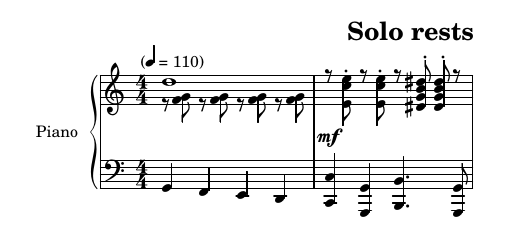
\includegraphics{../graphics/TheSoloRestsProblem.png}

\caption{The solo rests problem}
\label{The solo rests problem}
\end{center}
\end{figure}


% -------------------------------------------------------------------------
\section{Linear versus time-oriented representation}\label{Linear versus time-oriented representation}
% -------------------------------------------------------------------------

Most music scoring GUI applications handle music as containing voices, which are made of sequences of notes, chords, tuplets and such. This is a horizontal, linear view of the music in the score.

Another view of the music is time-oriented, i.e., what are are notes being played at a given moment in time? This is a vertical view of the music, which is highlighted in piano roll views.

MSR stores descriptions of so-called 'measures slice' through \class{msrMeasuresSlice}, defined in \msr{msrMeasuresSlice.h}. Then a time-oriented view of a voice, staff or part is a sequence of such measure slices, defined in \class{msrMeasuresSlicesSequence}.%%%JMI

An \class{msrMeasuresSlice} contains basically a slice measures vector:
\begin{lstlisting}[language=CPlusPlus]
    // the measures in the slice
    std::vector<S_msrMeasure>  fSliceMeasuresVector;
\end{lstlisting}

From this, the following other descriptions are derived:
\begin{lstlisting}[language=CPlusPlus]
    // notes flat list
    std::list<S_msrNote>  fSliceNotesFlatList;

    // note events list
    std::list<S_msrNoteEvent>
                          fSliceNoteEventsList;

    // simultaneous notes chunks list
    std::list<S_msrSimultaneousNotesChunk>
                          fSliceSimultaneousNotesChunksList;
\end{lstlisting}

Note events are distinguished with \enumType{msrNoteEventKind}:
\begin{lstlisting}[language=CPlusPlus]
//________________________________________________________________________
enum class msrNoteEventKind {
  kNoteEventStart,
  kNoteEventStop
};
\end{lstlisting}

\Class{msrNoteEvent} contains:
\begin{lstlisting}[language=CPlusPlus]
    mfRational              fNoteEventMeasurePosition;
    S_msrNote             fNoteEventNote;
    msrNoteEventKind      fNoteEventKind;

\end{lstlisting}

%%%JMI


% -------------------------------------------------------------------------
\section{Spanners}\label{Spanners}
% -------------------------------------------------------------------------

A spanner... spans from one note or rest to another one. A choice to be made about when to use spanners: should
wedges {\tt <} and {\tt >} be handled as spanners, or simply as being attached to notes? It has been selected to use spanners only for ligatures apart from true spanners.

\mxml\ uses {\tt "start"}, {\tt "start"} and {\tt "start"} attributes, which need to be present in MSR for \mxml\ generation. They are reflected in MSR as enumeration type \enumType{msrSpannerTypeKind}, defined this way:
\begin{lstlisting}[language=CPlusPlus]
// spanner types
//______________________________________________________________________________
enum class msrSpannerTypeKind {
  kSpannerType_UNKNOWN_,

  kSpannerTypeStart, kSpannerTypeContinue, kSpannerTypeStop
};
\end{lstlisting}


% -------------------------------------------------------------------------
\section{Uplinks, direct uplinks and sidelinks}\label{Uplinks, direct uplinks and sidelinks}
% -------------------------------------------------------------------------

An \upLink\ is a direct pointer from one class instance to one that contains it. Some are are a link to the containing class instance, whilst others are \shortcut\ links higher in the graph for speed. For example, \class{msrNote} contains:
\begin{lstlisting}[language=CPlusPlus]
    // upLinks
    // ------------------------------------------------------

    S_msrMeasure          fNoteUpLinkToMeasure;

    S_msrChord            fNoteShortcutUpLinkToChord;

    S_msrGraceNotesGroup  fNoteShortcutUpLinkToGraceNotesGroup;

    S_msrTuplet           fNoteShortcutUpLinkToTuplet;
\end{lstlisting}

A \sideLink\ is used in ligatures and spanners, so that each end of the structure can reference the other one.

For example, \mf\ defines \enumType{msrLigatureKind} in \msr{msrLigatures.h}:
\begin{lstlisting}[language=CPlusPlus]
enum class msrLigatureKind {
  kLigatureNone,
  kLigatureStart, kLigatureContinue, kLigatureStop
};
\end{lstlisting}

\Class{msrLigature} contains:
\begin{lstlisting}[language=CPlusPlus]
  private:

    // sideLinks
    // ------------------------------------------------------
    S_msrLigature         fLigatureSideLinkToOtherEnd; // two-way
\end{lstlisting}

\EnumType{} is declared in \msr{msrSpanners.h}:
\begin{lstlisting}[language=CPlusPlus]
enum class msrSpannerKind {
  kSpannerDashes, kSpannerWavyLine
};
\end{lstlisting}


% -------------------------------------------------------------------------
\section{Printing descriptions}\label{Printing descriptions}
% -------------------------------------------------------------------------

There is a standard set of methods to print the contents of the descriptions in \mf\ to \standardOutput, depending on the granularity of the information to be displayed:
\begin{lstlisting}[language=CPlusPlus]
    void                  print (std::ostream& os) const override;

    std::string           asString () const override;
    std::string           asStringShort () const override;
\end{lstlisting}

There are also more specific methods such as:
\begin{lstlisting}[language=CPlusPlus]
    void                  printFull (std::ostream& os) const override;

    void                  printSummary (std::ostream& os) const override;
\end{lstlisting}

Note that:
\begin{itemize}
\item \virtualMethod{asString} produces a rather condensed view of the data to be displayed as part of a single line;
\item \virtualMethod{print} may produce its output on multiples lines, which always ends with an end of line.
\end{itemize}

Most classes in \mf\ can be printed with the {\tt <<} operator:
\begin{lstlisting}[language=CPlusPlus]
std::ostream& operator << (std::ostream& os, const S_msrElement& elt)
{
  if (elt) {
    elt->print (os);
  }
  else {
    os << "[NULL]" << std::endl;
  }

  return os;
}
\end{lstlisting}

In simple cases, \virtualMethod{print} merely calls \virtualMethod{asString}:
\begin{lstlisting}[language=CPlusPlus]
void msrElement::print (std::ostream& os) const
{
  os << asString () << std::endl;
}
\end{lstlisting}

All \virtualMethod{asString} methods produce an output of the form {\tt [...]}, in order to facilitate selecting the whole with a double click to help the user, since such output can be nested:
\begin{lstlisting}[language=CPlusPlus]
std::string msrTransposition::asString () const
{
  std::stringstream ss;

  ss <<
    "[Transposition" <<
    ", fTranspositionDiatonic = " << fTranspositionDiatonic <<
    ", fTranspositionChromatic = " << fTranspositionChromatic <<
    ", fTranspositionOctaveChange = " << fTranspositionOctaveChange <<
    ", fTranspositionDouble = " << fTranspositionDouble <<
    ", line " << fInputLineNumber <<
    ']';

  return ss.str ();
}
\end{lstlisting}

A typical sequence to produce indented output is:
\begin{lstlisting}[language=CPlusPlus]
void msrTransposition::print (std::ostream& os) const
{
  const int fieldWidth = 22;

  os <<
    "Transposition" <<
    ", line " << fInputLineNumber <<
    std::endl;

  ++gIndenter;

  os << std::left <<
    std::setw (fieldWidth) <<
    "fTranspositionDiatonic" << ": " << fTranspositionDiatonic <<
    std::endl <<
    std::setw (fieldWidth) <<
    "fTranspositionChromatic" << ": " << fTranspositionChromatic <<
    std::endl <<
    std::setw (fieldWidth) <<
    "fTranspositionOctaveChange" << ": " << fTranspositionOctaveChange <<
    std::endl <<
    std::setw (fieldWidth) <<
    "fTranspositionDouble" << ": " << fTranspositionDouble <<
    std::endl << std::endl;

  --gIndenter;
}
\end{lstlisting}

The main indented output streams are:
\begin{lstlisting}[language=CPlusPlus]
#define gOutput *gGlobalOutputIndentedOstream
#define gLog    *gGlobalLogIndentedOstream

\end{lstlisting}


% -------------------------------------------------------------------------
\section{Pitches}\label{Pitches}
% -------------------------------------------------------------------------

MSR handle diatonic, semitone and quarter tone pitches, defined in \msr{msrBasicTypes.h} as shown below.
All pitches data is represented internally as quater tones pitches, and conversions are done wherever needed.

\begin{lstlisting}[language=CPlusPlus]
// diatonic pitches
//______________________________________________________________________________
enum class msrDiatonicPitchKind {
  kDiatonicPitch_UNKNOWN_,

  // starting at C for LilyPond relative octave calculations
  kDiatonicPitchC,
  kDiatonicPitchD, kDiatonicPitchE, kDiatonicPitchF,
  kDiatonicPitchG, kDiatonicPitchA, kDiatonicPitchB
};
\end{lstlisting}

\begin{lstlisting}[language=CPlusPlus]
// semi tones pitches
//______________________________________________________________________________
enum class msrSemiTonesPitchKind {
  kSTP_NoSemiTonesPitch,

  kSTP_C_TripleFlat,
  kSTP_C_DoubleFlat, kSTP_C_Flat,
  kSTP_C_Natural,
  kSTP_C_Sharp, kSTP_C_DoubleSharp,
  kSTP_C_TripleSharp,

  kSTP_D_TripleFlat,
  kSTP_D_DoubleFlat, kSTP_D_Flat,
  kSTP_D_Natural,
  kSTP_D_Sharp, kSTP_D_DoubleSharp,
  kSTP_D_TripleSharp,

  kSTP_E_TripleFlat,
  kSTP_E_DoubleFlat, kSTP_E_Flat,
  kSTP_E_Natural,
  kSTP_E_Sharp, kSTP_E_DoubleSharp,
  kSTP_E_TripleSharp,

  kSTP_F_TripleFlat,
  kSTP_F_DoubleleFlat, kSTP_F_Flat,
  kSTP_F_Natural,
  kSTP_F_Sharp, kSTP_F_DoubleSharp,
  kSTP_F_TripleSharp,

  kSTP_G_TripleFlat,
  kSTP_G_DoubleFlat, kSTP_G_Flat,
  kSTP_G_Natural,
  kSTP_G_Sharp, kSTP_G_DoubleSharp,
  kSTP_G_TripleSharp,

  kSTP_A_TripleFlat,
  kSTP_A_DoubleFlat, kSTP_A_Flat,
  kSTP_A_Natural,
  kSTP_A_Sharp, kSTP_A_DoubleSharp,
  kSTP_A_TripleSharp,

  kSTP_B_TripleFlat,
  kSTP_B_DoubleFlat, kSTP_B_Flat,
  kSTP_B_Natural,
  kSTP_B_Sharp, kSTP_B_DoubleSharp,
  kSTP_B_TripleSharp
};
\end{lstlisting}

\begin{lstlisting}[language=CPlusPlus]
// quarter tones pitches
//______________________________________________________________________________
enum class msrQuarterTonesPitchKind {
  kQTP_UNKNOWN_,

  kQTP_Rest, kQTP_Skip,

  kQTP_A_TripleFlat,
  kQTP_A_DoubleFlat, kQTP_A_SesquiFlat, kQTP_A_Flat, kQTP_A_SemiFlat,
  kQTP_A_Natural,
  kQTP_A_SemiSharp, kQTP_A_Sharp, kQTP_A_SesquiSharp, kQTP_A_DoubleSharp,
  kQTP_A_TripleSharp,

  kQTP_B_TripleFlat,
  kQTP_B_DoubleFlat, kQTP_B_SesquiFlat, kQTP_B_Flat, kQTP_B_SemiFlat,
  kQTP_B_Natural,
  kQTP_B_SemiSharp, kQTP_B_Sharp, kQTP_B_SesquiSharp, kQTP_B_DoubleSharp,
  kQTP_B_TripleSharp,

  kQTP_C_TripleFlat,
  kQTP_C_DoubleFlat, kQTP_C_SesquiFlat, kQTP_C_Flat, kQTP_C_SemiFlat,
  kQTP_C_Natural,
  kQTP_C_SemiSharp, kQTP_C_Sharp, kQTP_C_SesquiSharp, kQTP_C_DoubleSharp,
  kQTP_C_TripleSharp,

  kQTP_D_TripleFlat,
  kQTP_D_DoubleFlat, kQTP_D_SesquiFlat, kQTP_D_Flat, kQTP_D_SemiFlat,
  kQTP_D_Natural,
  kQTP_D_SemiSharp, kQTP_D_Sharp, kQTP_D_SesquiSharp, kQTP_D_DoubleSharp,
  kQTP_D_TripleSharp,

  kQTP_E_TripleFlat,
  kQTP_E_DoubleFlat, kQTP_E_SesquiFlat, kQTP_E_Flat, kQTP_E_SemiFlat,
  kQTP_E_Natural,
  kQTP_E_SemiSharp, kQTP_E_Sharp, kQTP_E_SesquiSharp, kQTP_E_DoubleSharp,
  kQTP_E_TripleSharp,

  kQTP_F_TripleFlat,
  kQTP_F_DoubleFlat, kQTP_F_SesquiFlat, kQTP_F_Flat, kQTP_F_SemiFlat,
  kQTP_F_Natural,
  kQTP_F_SemiSharp, kQTP_F_Sharp, kQTP_F_SesquiSharp, kQTP_F_DoubleSharp,
  kQTP_F_TripleSharp,

  kQTP_G_TripleFlat,
  kQTP_G_DoubleFlat, kQTP_G_SesquiFlat, kQTP_G_Flat, kQTP_G_SemiFlat,
  kQTP_G_Natural,
  kQTP_G_SemiSharp, kQTP_G_Sharp, kQTP_G_SesquiSharp, kQTP_G_DoubleSharp,
  kQTP_G_TripleSharp
};
\end{lstlisting}


% -------------------------------------------------------------------------
\section{Octaves}\label{Octaves}
% -------------------------------------------------------------------------

They are represented with enumeration type {\tt }:
\begin{lstlisting}[language=CPlusPlus]
// octaves
//______________________________________________________________________________
enum class msrOctaveKind {
  kOctave_UNKNOWN_,

  kOctave0, kOctave1, kOctave2, kOctave3,
  kOctave4, // that of middle C
  kOctave5, kOctave6, kOctave7, kOctave8, kOctave9
};
\end{lstlisting}

For the needs of LilyPond and MSDL, MSR also contains a description of how to enter octaves:
\begin{lstlisting}[language=CPlusPlus]
// octave entry
//______________________________________________________________________________
enum class msrOctaveEntryKind {
  kOctaveEntryRelative,
  kOctaveEntryAbsolute,
  kOctaveEntryFixed
};
\end{lstlisting}


% -------------------------------------------------------------------------
\section{NotesDurations}\label{NotesDurations}
% -------------------------------------------------------------------------

They are represented in MSR with the \enumType{msrNotesDurationKind} enumeration type, defined in \msr{msrBasicTypes.h}:
\begin{lstlisting}[language=CPlusPlus]
// durations
//______________________________________________________________________________
enum class msrNotesDurationKind {
  kNotesDuration_UNKNOWN_,

  // from longest to shortest for the algorithms
  kNotesDurationMaxima, kNotesDurationLonga, kNotesDurationBreve, kNotesDurationWhole, kNotesDurationHalf,
  kNotesDurationQuarter,
  kNotesDurationEighth, kNotesDuration16th, kNotesDuration32nd, kNotesDuration64th, kNotesDuration128th, kNotesDuration256th, kNotesDuration512th, kNotesDuration1024th
};
\end{lstlisting}

\Class{msrDottedNotesDuration} contains:
\begin{lstlisting}[language=CPlusPlus]
    msrNotesDurationKind  fNotesDurationKind;
    int                   fDotsNumber;
\end{lstlisting}


% -------------------------------------------------------------------------
\section{Alterations}\label{Alterations}
% -------------------------------------------------------------------------

\begin{lstlisting}[language=CPlusPlus]
// alterations
//______________________________________________________________________________
enum class msrAlterationKind {
  kAlteration_UNKNOWN_,

  kAlterationTripleFlat, kAlterationDoubleFlat, kAlterationSesquiFlat,
  kAlterationFlat, kAlterationSemiFlat,
  kAlterationNatural,
  kAlterationSemiSharp, kAlterationSharp, kAlterationSesquiSharp,
  kAlterationDoubleSharp, kAlterationTripleSharp
\end{lstlisting}


% -------------------------------------------------------------------------
\section{Accidentals}\label{Accidentals}
% -------------------------------------------------------------------------

\begin{lstlisting}[language=CPlusPlus]
// accidentals
//______________________________________________________________________________
enum class msrAccidentalKind {
  kAccidentalNone,

  kAccidentalSharp, kAccidentalNatural,
  kAccidentalFlat, kAccidentalDoubleSharp,
  kAccidentalSharpSharp,
  kAccidentalFlatFlat, kAccidentalNaturalSharp,
  kAccidentalNaturalFlat, kAccidentalQuarterFlat,
  kAccidentalQuarterSharp,kAccidentalThreeQuartersFlat,
  kAccidentalThreeQuartersSharp,

  kAccidentalSharpDown, kAccidentalSharpUp,
  kAccidentalNaturalDown, kAccidentalNaturalUp,
  kAccidentalFlatDown, kAccidentalFlatUp,
  kAccidentalTripleSharp, kAccidentalTripleFlat,
  kAccidentalSlashQuarterSharp, kAccidentalSlashSharp,
  kAccidentalSlashFlat, kAccidentalDoubleSlashFlat,
  kAccidentalSharp_1, kAccidentalSharp_2,
  kAccidentalSharp_3,  kAccidentalSharp_5,
  kAccidentalFlat_1, kAccidentalFlat_2,
  kAccidentalFlat_3, kAccidentalFlat_4,
  kAccidentalSori, kAccidentalKoron,

  kAccidentalOther
};
\end{lstlisting}


% -------------------------------------------------------------------------
\section{Tempos}\label{Tempos}
% -------------------------------------------------------------------------

There are thus several kinds of tempos in \msrRepr, with variants represented by \enumType{msrTempoKBeatUnitsKind} in \msr{msrTempos.h}:
\begin{lstlisting}[language=CPlusPlus]
class EXP msrTempo : public msrMeasureElement
{
  public:

    // data types
    // ------------------------------------------------------

    enum class msrTempoKBeatUnitsKind {
      kTempoBeatUnits_UNKNOWN_,
      kTempoBeatUnitsWordsOnly,
      kTempoBeatUnitsPerMinute,
      kTempoBeatUnitsEquivalence,
      kTempoNotesRelationship
    };

		// ... ... ...

    enum class msrTempoParenthesizedKind {
      kTempoParenthesizedYes, kTempoParenthesizedNo
    };

		// ... ... ...

    enum class msrTempoNotesRelationshipKind {
      kTempoNotesRelationshipNone, kTempoNotesRelationshipEquals
    };

		// ... ... ...
};
\end{lstlisting}


% -------------------------------------------------------------------------
\subsection{Tempos notes}\label{Tempos notes}
% -------------------------------------------------------------------------

A tempo indication can contain a note a notes in a tuplet. Such notes are described by \class{msrTempoNote}:
\begin{lstlisting}[language=CPlusPlus]
class EXP msrTempoNote : public msrElement
{
  public:

    // creation from MusicXML
    // ------------------------------------------------------

    static SMARTP<msrTempoNote> create (
                            int             inputLineNumber,
                            const mfRational& tempoNoteWholeNotes,
                            Bool            tempoNoteBelongsToATuplet);

  protected:

    // constructors/destructor
    // ------------------------------------------------------

                          msrTempoNote (
                            int             inputLineNumber,
                            const mfRational& tempoNoteWholeNotes,
                            Bool            tempoNoteBelongsToATuplet);

		// ... ... ...

  private:

    // private fields
    // ------------------------------------------------------

    mfRational              fTempoNoteWholeNotes;

    std::list<S_msrBeam>  fTempoNoteBeams;

    Bool                  fTempoNoteBelongsToATuplet;
};
\end{lstlisting}

% -------------------------------------------------------------------------
\subsection{Tempos tuplets}\label{Tempos tuplets}
% -------------------------------------------------------------------------

A tuplet in a tempo representation is described by \class{msrTempoTuplet}:
\begin{lstlisting}[language=CPlusPlus]
//______________________________________________________________________________
class EXP msrTempoTuplet : public msrElement
{
  public:

    // data types
    // ------------------------------------------------------

    enum class msrTempoTupletTypeKind {
      kTempoTupletTypeNone,
      kTempoTupletTypeStart, kTempoTupletTypeStop
    };

		// ... ... ...

    enum class msrTempoTupletBracketKind {
      kTempoTupletBracketYes, kTempoTupletBracketNo
    };

		// ... ... ...

    enum class msrTempoTupletShowNumberKind {
      kTempoTupletShowNumberActual,
      kTempoTupletShowNumberBoth,
      kTempoTupletShowNumberNone
    };

		// ... ... ...

    // creation from MusicXML
    // ------------------------------------------------------

    static SMARTP<msrTempoTuplet> create (
      int                          inputLineNumber,
      int                          tempoTupletNumber,
      msrTempoTupletBracketKind    tempoTupletBracketKind,
      msrTempoTupletShowNumberKind tempoTupletShowNumberKind,
      msrTupletFactor              tempoTupletFactor,
      msrWholeNotes            memberNotesDisplayWholeNotes);

  protected:

    // constructors/destructor
    // ------------------------------------------------------

    msrTempoTuplet (
      int                          inputLineNumber,
      int                          tempoTupletNumber,
      msrTempoTupletBracketKind    tempoTupletBracketKind,
      msrTempoTupletShowNumberKind tempoTupletShowNumberKind,
      msrTupletFactor              tempoTupletFactor,
      msrWholeNotes            memberNotesDisplayWholeNotes);

		// ... ... ...

  private:

    // private fields
    // ------------------------------------------------------

    int                   fTempoTupletNumber;

    msrTempoTupletBracketKind
                          fTempoTupletBracketKind;

    msrTempoTupletShowNumberKind
                          fTempoTupletShowNumberKind;

    msrTupletFactor       fTempoTupletFactor;

    mfRational              fMemberNotesDisplayWholeNotes;

    mfRational              fTempoTupletDisplayWholeNotes;

    std::list<S_msrElement>
                          fTempoTupletElements;
};
\end{lstlisting}


% -------------------------------------------------------------------------
\subsection{Tempos description}\label{Tempos description}
% -------------------------------------------------------------------------

The private fields in \class{msrTempo} are:
\begin{lstlisting}[language=CPlusPlus]
class EXP msrTempo : public msrMeasureElement
{
	// ... ... ...

  private:

    // private fields
    // ------------------------------------------------------

    msrTempoKBeatUnitsKind
                          fTempoKind;

    std::list<S_msrWords> fTempoWordsList;

    msrDottedNotesDuration     fTempoBeatUnit;

    std::string           fTempoPerMinute; // '90' or '132-156' for example
    msrDottedNotesDuration     fTempoEquivalentBeatUnit;

    S_msrTempoNotesRelationshipElements
                          fTempoNotesRelationshipLeftElements;
    msrTempoNotesRelationshipKind
                          fTempoNotesRelationshipKind;
    S_msrTempoNotesRelationshipElements
                          fTempoNotesRelationshipRightElements;

    msrTempoParenthesizedKind
                          fTempoParenthesizedKind;

    msrPlacementKind      fTempoPlacementKind;
};
\end{lstlisting}

Among these fields:
\begin{itemize}
\item \field{msrTempo}{fTempoKind} denotes the variant;
\item \field{msrTempo}{fTempoWordsList} contains the words that can be present, such as 'adagio molto';
\item \field{msrTempo}{fTempoBeatUnit} is a dotted duration, as in '4.';
\item \field{msrTempo}{fTempoPerMinute} is a std::string, since it can contain ranges indication as in '4. = 60-66';
\item \field{msrTempo}{fTempoEquivalentBeatUnit} is a dotted duration; %%%JMI
\item \field{msrTempo}{fTempoNotesRelationshipLeftElements}, \field{msrTempo}{fTempoNotesRelationshipKind} and \field{msrTempo}{fTempoNotesRelationshipRightElements} are used when a relationship is present, such as '2. = 1', in which case \field{msrTempo}{fTempoNotesRelationshipKind} contains \field{msrTempo}{kTempoNotesRelationshipEquals};
\item \field{msrTempo}{fTempoParenthesizedKind} indicates whether the tempo indication is parenthesized;
\item \field{msrTempo}{fTempoPlacementKind} tells whether the tempo is to be places above or below the staff, \constant{msrPlacementKind}{kPlacementAbove} by default.
\end{itemize}


% -------------------------------------------------------------------------
\section{Clefs}\label{Clefs}
% -------------------------------------------------------------------------

Clefs are distinguished using \enumType{msrClefKind}:
\begin{lstlisting}[language=CPlusPlus]
// clefs
//______________________________________________________________________________

enum class msrClefKind {
  kClef_UNKNOWN_,

  kClefTreble,
  kClefSoprano, kClefMezzoSoprano, kClefAlto, kClefTenor, kClefBaritone, kClefBass,
  kClefTrebleLine1,
  kClefTrebleMinus15, kClefTrebleMinus8, kClefTreblePlus8, kClefTreblePlus15,

  kClefBassMinus15, kClefBassMinus8, kClefBassPlus8, kClefBassPlus15,

  kClefVarbaritone,

  kClefTablature4, kClefTablature5, kClefTablature6, kClefTablature7,

  kClefPercussion,

  kClefJianpu
};
\end{lstlisting}

\Class{msrClef} contains:
\begin{lstlisting}[language=CPlusPlus]
    msrClefKind           fClefKind;
    int                   fClefStaffNumber;
\end{lstlisting}


% -------------------------------------------------------------------------
\section{Keys}\label{Keys}
% -------------------------------------------------------------------------

MSR, as \mxml, suports Humdrum-Scot keys as well as traditional key such as {\tt C} and {\tt 6/8}.

A Humdrum-Scot key is composed of items represented by \class{msrHumdrumScotKeyItem}, each containing:
\begin{lstlisting}[language=CPlusPlus]
    msrDiatonicPitchKind  fKeyDiatonicPitchKind;
    msrAlterationKind     fKeyAlterationKind;
    msrOctaveKind         fKeyOctaveKind;
\end{lstlisting}

An example is at \figureRef{Humdrum-Scot keys}. It has been produced by:
\begin{lstlisting}[language=Terminal]
xml2ly -auto-output-file-name keys/HumdrumScotKeys.xml
\end{lstlisting}

\begin{figure}[htbp]
\begin{center}
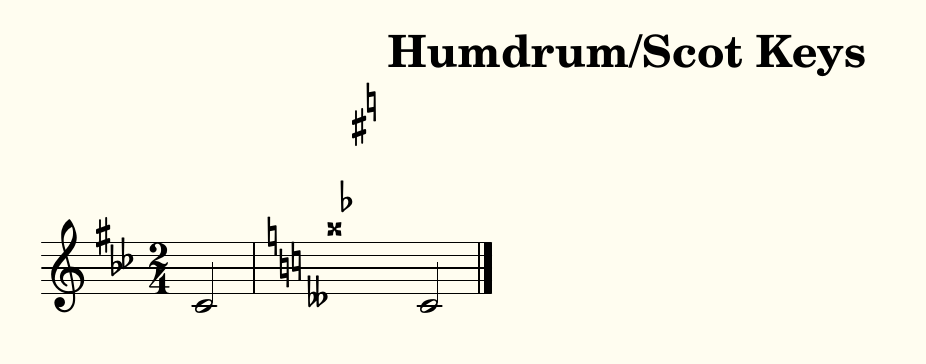
\includegraphics{../graphics/HumdrumScotKeys.png}

\caption{Humdrum-Scot keys}
\label{Humdrum-Scot keys}
\end{center}
\end{figure}

\Class{msrKey} thus contains:
\begin{lstlisting}[language=CPlusPlus]
    // private fields
    // ------------------------------------------------------

    msrKeyKind            fKeyKind;

    // traditional keys

    msrQuarterTonesPitchKind
                          fKeyTonicQuarterTonesPitchKind;
    msrModeKind           fModeKind;
    int                   fKeyCancel;

    // Humdrum/Scot keys

    std::vector<S_msrHumdrumScotKeyItem>
                          fHumdrumScotKeyItemsVector;
    Bool                  fKeyItemsOctavesAreSpecified;
\end{lstlisting}


% -------------------------------------------------------------------------
\section{Time signatures}\label{Time signatures}
% -------------------------------------------------------------------------

The variants in time signatures are distinguished by enumeration type \enumType{msrTimeSignatureSymbolKind}:
\begin{lstlisting}[language=CPlusPlus]
// time symbols
//______________________________________________________________________________
enum class msrTimeSignatureSymbolKind {
  kTimeSignatureSymbolNone,
  kTimeSignatureSymbolCommon,
  kTimeSignatureSymbolCut,
  kTimeSignatureSymbolNote,
  kTimeSignatureSymbolDottedNote,
  kTimeSignatureSymbolSingleNumber,
  kTimeSignatureSymbolSenzaMisura
};
\end{lstlisting}

A time signature can also be structured, and this is described by those two types:
\begin{lstlisting}[language=CPlusPlus]
enum class msrTimeSignatureSeparatorKind {
  kTimeSignatureSeparatorNone,
  kTimeSignatureSeparatorHorizontal,
  kTimeSignatureSeparatorDiagonal,
  kTimeSignatureSeparatorVertical,
  kTimeSignatureSeparatorAdjacent
};
\end{lstlisting}

\begin{lstlisting}[language=CPlusPlus]
enum class msrTimeSignatureRelationKind {
  kTimeSignatureRelationNone,
  kTimeSignatureRelationParentheses,
  kTimeSignatureRelationBracket,
  kTimeSignatureRelationEquals,
  kTimeSignatureRelationSlash,
  kTimeSignatureRelationSpace,
  kTimeSignatureRelationHyphen
};
\end{lstlisting}

A brick that can be used in \class{msrTimeSignature} is {\tt msrTimeSignatureItem}, whose private fields are:
\begin{lstlisting}[language=CPlusPlus]
    std::vector<int>      fTimeSignatureBeatsNumbersVector; // 5+3+1 is possible
    int                   fTimeSignatureBeatValue;
\end{lstlisting}

\Class{msrTimeSignature} contains:
\begin{lstlisting}[language=CPlusPlus]
    msrTimeSignatureSymbolKind
                          fTimeSignatureSymbolKind;

    std::vector<S_msrTimeSignatureItem>
                          fTimeSignatureItemsVector;

    // a time is compound if it contains several items
    // or if the only one has several beats numbers
    // i.e. 3/4 is not, (3+4)/8 is, and 2/4+3/4 is too
    Bool                  fTimeIsCompound;
\end{lstlisting}


% -------------------------------------------------------------------------
\section{MSR classes inheritance}\label{MSR classes inheritance}
% -------------------------------------------------------------------------

The picture at \figureRef{The MSR classes hierarchy}, shows the hierarchy of the main MSR classes. The  colors are used as follows:

\subimport{../CommonLaTeXFiles}{MSRClassesHierarchyPicture}

The background colors are used as follows:
\begin{itemize}
\item \colorbox{black}{\textcolor{green}{green}}: a score element that is expected to be found in a score representation, such as \class{msrStaff} and \class{msrChord};

\item \colorbox{black}{\textcolor{pink}{pink}}: a element needed in MSR to structure the representation, such as \class{msrSegment} and \class{msrSyllable};

\item \colorbox{black}{\textcolor{yellow}{yellow}}: a base class   with name \class{msr*Element} for elements that can be used in another class, such as \class{msrVoiceElement};
\end{itemize}

The arrows colors have the following meaning:
\begin{itemize}
\item \textcolor{red}{red}: a link from a class   to its base class. For example, \class{msrPart} is derived from \class{msrPartGroupElement}, \class{msrPartGroup} is derived from \class{msrPartGroupElement}, and \class{msrChord} is derived from \class{msrTupletElement};

\item \textcolor{blue}{blue}: one or more fields of a class   are smart pointers to instances of another. For example, an \class{msrChords} instance may be an element of a \class{msrGraceNotesGroup} instance.
\end{itemize}

When not shown for clarity, the common base class   of all these classes is \class{msrElement}, that contains an integer input line number.

The {\tt otherMeasureElements} classes are:
\begin{itemize}
\item bars:

\begin{itemize}
  \item \class{msrBarCheck}
  \item \class{msrBarNumberCheck}
  \item \class{msrBarLine}
  \item \class{msrHiddenMeasureAndBarLine}
  \end{itemize}

\item breaks:

\begin{itemize}
  \item \class{msrLineBreak}
  \item \class{msrPageBreak}
  \end{itemize}

\item notes:

\begin{itemize}
  \item \class{msrVoiceStaffChange}
  \item \class{msrOctaveShift}
  \end{itemize}

\item clefs, keys, times, tempo:

\begin{itemize}
  \item \class{msrClef}
  \item \class{msrKey}
  \item \class{msrTime}
  \item \class{msrTempo}
  \end{itemize}

\item instruments:

\begin{itemize}
  \item \class{msrStaffDetails}
  \item \class{msrScordatura}
  \item \class{msrAccordionRegistration}
  \item \class{msrHarpPedalsTuning}
  \item \class{msrPedal}
  \item \class{msrDamp}
  \item \class{msrDampAll}
  \end{itemize}

\item lyrics:

\begin{itemize}
	\item \class{msrSyllable}
  \end{itemize}

\item rehearsals, segno and coda:

\begin{itemize}
  \item \class{msrRehearsalMark}
	\item \class{msrSegno}
  \item \class{msrDalSegno}
  \item \class{msrCoda}
 \end{itemize}

\item others:

\begin{itemize}
  \item \class{msrPrintLayout}
  \item \class{msrEyeGlasses}
  \item \class{msrStaffLevelElement}
  \item \class{msrTransposition}
  \item \class{msrTupletElement}
  \end{itemize}

\end{itemize}


% -------------------------------------------------------------------------
\section{Books}\label{Books}
% -------------------------------------------------------------------------

Books handling is presented at \sectionRef{Books handling}.

\lily\ handles \lilycmd{book} by placing the scores one after the other in the resulting PDF or SVG files. It will also generate separate MIDI files if a \lilycmd{markup} block is used.

There is no such concept in MusicXML, but MSR uses it for completeness, creating an implicit \class{msrBook} instance if needed.

An \class{msrBook} contains a list and a set of {\tt S_msrBookElement}:
\begin{lstlisting}[language=CPlusPlus]
    // book elements
    std::set<S_msrBookElement> fBookElementsSet;

    std::list<S_msrBookElement>fBookElementsList;
\end{lstlisting}

Currently, the only book element used is the \class{msrScore}, but others might come, such as texts, which \lily\ allows as \lilycmd{markup}:
\begin{lstlisting}[language=Terminal]
jacquesmenu@macmini: ~/musicformats-git-dev/src > grep -r 'public msrBook' *
formats/msr/msrScores.h:class EXP msrScore : public msrBookElement
\end{lstlisting}


% -------------------------------------------------------------------------
\section{Scores}\label{Scores}
% -------------------------------------------------------------------------

Scores handling is presented at \sectionRef{Scores handling}.

A score in MSR is the usual music score concept. It contains a set and a list of {\tt S_msrPartGroup}:
\begin{lstlisting}[language=CPlusPlus]
    // part groups
    std::set<S_msrPartGroup>   fScorePartGroupsSet;

    std::list<S_msrPartGroup>  fPartGroupsList;
\end{lstlisting}


% -------------------------------------------------------------------------
\section{Part groups}\label{Part groups}
% -------------------------------------------------------------------------

Part groups handling is presented at \sectionRef{Part groups handling}.

A part group in MSR contains parts or other part groups. This concept is recursive, as it is in music score: the winds part group can oboes and horns part group, for example.
An implicit part group exists in MSR if the score does not contain explicit part groups.

An \class{msrPartGroup} thus contains parts and part groups in any order, as is found in symphonic music scores:
\begin{lstlisting}[language=Terminal]
jacquesmenu@macmini: ~/musicformats-git-dev/src > grep -r 'public msrPartGroupElement' *
formats/msr/msrParts.h:class EXP msrPart : public msrPartGroupElement
formats/msr/msrPartGroups.h:class EXP msrPartGroup : public msrPartGroupElement
\end{lstlisting}

which are stored in a list:
\begin{lstlisting}[language=CPlusPlus]
    // allowing for both parts and (sub-)part groups as elements
    std::list<S_msrPartGroupElement>
                          fPartGroupElementsList;
\end{lstlisting}


% -------------------------------------------------------------------------
\section{Parts}\label{Parts}
% -------------------------------------------------------------------------

Parts handling is presented at \sectionRef{Parts handling}.

A part in MSR is composed of voices, stored in:
\begin{lstlisting}[language=CPlusPlus]
    // staves

    std::map<int, S_msrStaff>
                          getPartStaveNumbersToStavesMap;
    std::list<S_msrStaff> fPartAllStavesList;

    // harmonies

    S_msrStaff            fPartHarmoniesStaff;
    S_msrVoice            fPartHarmoniesVoice;

    // figured bass

    S_msrStaff            fPartFiguredBassStaff;
    S_msrVoice            fPartFiguredBassVoice;

    // voices

    std::list<S_msrVoice> fPartAllVoicesList;
\end{lstlisting}


% -------------------------------------------------------------------------
\section{Staves}\label{Staves}
% -------------------------------------------------------------------------

Staves handling is presented at \sectionRef{Staves handling}.

A stave contains at most 4 numbered voices, stored in:
\begin{lstlisting}[language=CPlusPlus]
    // the mapping of all the voices in the staff,
    // including harmonies and figured bass voices
    std::map<int, S_msrVoice>
                          fStaffVoiceNumbersToAllVoicesMap;

    // the mapping of voice numbers to regular voices
    std::map<int, S_msrVoice>
                          fStaffVoiceNumbersToRegularVoicesMap;

    // we need to handle the regular voice specifically
    // to assign them sequencing numbers from 1 to gMaxStaffVoices,
    // needed to set the beams orientation (up or down)
    int                   fStaffRegularVoicesCounter;

    // harmonies and figured bass elements should be placed %%%JMI
    // in the first regular voice of the staff, hence:
    std::list<S_msrVoice> fStaffRegularVoicesList;

    // we need to sort the voices by increasing voice numbers,
    // but with harmonies voices right before the corresponding regular voices
    std::list<S_msrVoice> fStaffAllVoicesList;
\end{lstlisting}


% -------------------------------------------------------------------------
\section{Voice elements}\label{Voice elements}
% -------------------------------------------------------------------------

Voices contain instances of \class{msrVoiceElement}, defined in \msrBoth{msrVoiceElements}:
\begin{lstlisting}[language=CPlusPlus]
//______________________________________________________________________________
/*
  Various elements can found in voices,
  hence class   msrVoiceElement
*/

class EXP msrVoiceElement : public msrElement
{
  public:

    // creation from MusicXML
    // ------------------------------------------------------

    // cloning
    // ------------------------------------------------------

  protected:

                          msrVoiceElement (
                            int inputLineNumber);

    virtual               ~msrVoiceElement ();

  /*
    The voice uplink is declared in the sub-classes,
    to allow for separate *.h files, C++ constraint
  */
};
\end{lstlisting}

The classes derived from \class{msrVoiceElement} are:
\begin{lstlisting}[language=Terminal]
jacquesmenu@macmini: ~/musicformats-git-dev/src/formats/msr > grep 'public msrVoiceElement' *.h
msrBeatRepeats.h:class EXP msrBeatRepeat : public msrVoiceElement
msrMeasureRepeats.h:class EXP msrMeasureRepeat : public msrVoiceElement
msrRepeats.h:class EXP msrRepeat : public msrVoiceElement
msrMultipleFullBarRests.h:class EXP msrMultipleFullBarRests : public msrVoiceElement
msrSegments.h:class EXP msrSegment : public msrVoiceElement
\end{lstlisting}

They are describes in specific sections below.


% -------------------------------------------------------------------------
\section{Voices}\label{Voices}
% -------------------------------------------------------------------------

Voices handling is presented at \sectionRef{Voices handling}.

A voice is conceptually a sequence of {\tt S_msrVoiceElement}, that may be:
\begin{lstlisting}[language=Terminal]
jacquesmenu@macmini: ~/musicformats-git-dev/src > grep -r 'public msrVoiceElement' *
formats/msr/msrMeasureRepeats.h:class EXP msrMeasureRepeat : public msrVoiceElement
formats/msr/msrRepeats.h:class EXP msrRepeat : public msrVoiceElement
formats/msr/msrMultipleFullBarRests.h:class EXP msrMultipleFullBarRests : public msrVoiceElement
formats/msr/msrBeatRepeats.h:class EXP msrBeatRepeat : public msrVoiceElement
formats/msr/msrSegments.h:class EXP msrSegment : public msrVoiceElement
\end{lstlisting}

More precisely and for technical reasons, an \class{msrVoice} contains:
\begin{lstlisting}[language=CPlusPlus]
    // voice initial elements list

    std::list<S_msrVoiceElement>
                          fVoiceInitialElementsList;

    // voice first and last segments

    // fVoiceLastSegment contains the music
    // not yet stored in fVoiceInitialElementsList,
    // it is thus logically the end of the latter,
    // and is created implicitly for every voice.
    // It is needed 'outside' of the 'list<S_msrElement>'
    // because it is not a mere S_msrElement, but a S_msrSegment
    S_msrSegment          fVoiceLastSegment;

    // fVoiceFirstSegment is used to work around LilyPond issue #34
    S_msrSegment          fVoiceFirstSegment;
\end{lstlisting}

Each voice is described by a field of \enumType{msrVoiceKind}, defined in\\
\msr{msrBasicTypes.h}:
\begin{lstlisting}[language=CPlusPlus]
enum class msrVoiceKind {
  kVoiceKindRegular,
  kVoiceKindDynamics,
  kVoiceKindHarmonies,  // for MusicXML <harmony/>, LilyPond ChordNames
  kVoiceKindFiguredBass // for MusicXML <figured-bass/>, LilyPond FiguredBass
};
\end{lstlisting}

As stated in the comment above, {\tt fVoiceLastSegment} is used because it because {\tt fVoiceInitialElementsList} can contain any \class{msrVoiceElement}, whereas all \msrRepr\ elements appended to the voice are to be placed in a segment.

An \class{msrSegment} instance should thus be created and stored in {\tt fVoiceLastSegment} before \class{msrVoiceElement} instances can be appended to the voice.

When repeats are handled, an \class{msrRepeat} instance is created. Then the contents of \field{msrVoice}{fVoiceLastSegment} is moved into it and a new segment is created, see \sectionRef{Repeats}.%%%JMI

Wether the last segment should be created right when the voice is created is controlled with \enumType{msrVoiceCreateInitialLastSegmentKind}, defined in \msr{msrVoices.h}:
\begin{lstlisting}[language=CPlusPlus]
enum class msrVoiceCreateInitialLastSegmentKind {
  kCreateInitialLastSegmentYes,
  kCreateInitialLastSegmentNo
};
\end{lstlisting}


% -------------------------------------------------------------------------
\section{Measures}\label{Measures}
% -------------------------------------------------------------------------

Measures handling is presented at \sectionRef{Measures handling}.

A measure is a linear, flat sequence of \class{msrMeasureElements}, some of which are structured, such as \class{msrChord}. \Class{msrMeausre} is defined in \msrBoth{msrMeausre}.

The measure elements are defined in \msr{}:
\begin{lstlisting}[language=Terminal]
jacquesmenu@macmini: ~/musicformats-git-dev/src/formats/msr > grep  'public msrMeasureElement' *.h
msrBars.h:class EXP msrBarCheck : public msrMeasureElement
msrBars.h:class EXP msrBarNumberCheck : public msrMeasureElement
msrBars.h:class EXP msrBarLine : public msrMeasureElement
msrBreaks.h:class EXP msrLineBreak : public msrMeasureElement
msrBreaks.h:class EXP msrPageBreak : public msrMeasureElement
msrClefs.h:class EXP msrClef : public msrMeasureElement
msrCodas.h:class EXP msrCoda : public msrMeasureElement
msrDoubleTremolos.h:class EXP msrDoubleTremolo : public msrMeasureElement
msrEyeGlasses.h:class EXP msrEyeGlasses : public msrMeasureElement
msrFiguredBasses.h:class EXP msrFiguredBass : public msrMeasureElement
msrHarmonies.h:class EXP msrHarmony : public msrMeasureElement
msrHiddenMeasureAndBarLines.h:class EXP msrHiddenMeasureAndBarLine : public msrMeasureElement
msrInstruments.h:class EXP msrScordatura : public msrMeasureElement
msrInstruments.h:class EXP msrAccordionRegistration : public msrMeasureElement
msrInstruments.h:class EXP msrHarpPedalsTuning : public msrMeasureElement
msrInstruments.h:class EXP msrPedal : public msrMeasureElement
msrInstruments.h:class EXP msrDamp : public msrMeasureElement
msrInstruments.h:class EXP msrDampAll : public msrMeasureElement
msrKeys.h:class EXP msrKey : public msrMeasureElement
msrLyrics.h:class EXP msrSyllable : public msrMeasureElement
msrMusicXMLSpecifics.h:class EXP msrPrintLayout : public msrMeasureElement
msrRehearsalMarks.h:class EXP msrRehearsalMark : public msrMeasureElement
msrSegnos.h:class EXP msrSegno : public msrMeasureElement
msrDalSegnos.h:class EXP msrDalSegno : public msrMeasureElement
msrStavesDetails.h:class EXP msrStaffDetails : public msrMeasureElement
msrTempos.h:class EXP msrTempo : public msrMeasureElement
msrTimeSignatures.h:class EXP msrTimeSignature : public msrMeasureElement
msrTranspositions.h:class EXP msrOctaveShift : public msrMeasureElement
msrTranspositions.h:class EXP msrTransposition : public msrMeasureElement
msrVoiceStaffChanges.h:class EXP msrVoiceStaffChange : public msrMeasureElement
\end{lstlisting}


In order to perform a time-wise analysis of the scores, MSR contains \class{msrmeasure} linear flat lists, without the \class{msrRepeat} and such being represented.\\
This is used when identifying rest notes that are not 'heard' simultaneously with other notes or rests: this way, the rest can ignore the current voice number and be placed in the vertical middle of the staff.

Apart from the cloning methods, only one method creates measures, namely\\
\method{msrSegment}{createAMeasureAndAppendItToSegment}, defined in\\
\msrBoth{msrSegments}:
\begin{lstlisting}[language=CPlusPlus]
S_msrMeasure msrSegment::createAMeasureAndAppendItToSegment (
  int    inputLineNumber,
  std::string measureNumber,
  msrMeasureImplicitKind
         measureImplicitKind)
{
	// ... ... ...

  ++gIndenter;

  // determine new measure 'first in segment' kind
  msrMeasureFirstInSegmentKind
    measureFirstInSegmentKind;

  if (fSegmentElementsList.size () == 0) {
    // this is the first measure in the segment
    measureFirstInSegmentKind =
      msrMeasureFirstInSegmentKind::kMeasureFirstInSegmentKindYes;
  }
  else {
    // this is not the first measure in the segment
    measureFirstInSegmentKind =
      msrMeasureFirstInSegmentKind::kMeasureFirstInSegmentKindNo;
  }

  // create a measure
	// ... ... ...

  S_msrMeasure
    result =
      msrMeasure::create (
        inputLineNumber,
        measureNumber,
        this);

  // set result's ordinal number
  result->
    setMeasureOrdinalNumberInVoice (
      fSegmentUpLinkToVoice->
        incrementVoiceCurrentMeasureOrdinalNumber ());

  // append result to the segment
  appendMeasureToSegment (result);

  --gIndenter;

  return result;
}
\end{lstlisting}


% -------------------------------------------------------------------------
\section{Repeats patterns and replicas}\label{Repeats patterns and replicas}
% -------------------------------------------------------------------------

\msrRepr\ represents repeated beats and measures this way:
\begin{itemize}
\item a pattern describes what is repeated;
\item there are as many replicas of the music as needed.
\end{itemize}

This leads to:
\begin{lstlisting}[language=Terminal]
jacquesmenu@macmini: ~/musicformats-git-dev/src/formats/msr > grep Pattern *.h | grep class
msrBeatRepeats.h:class EXP msrBeatRepeatPattern : public msrElement
msrMeasureRepeats.h:class EXP msrMeasureRepeatPattern : public msrElement
jacquesmenu@macmini: ~/musicformats-git-dev/src/formats/msr > grep Replicas *.h | grep class
msrBeatRepeats.h:class EXP msrBeatRepeatReplicas : public msrElement
msrMeasureRepeats.h:class EXP msrMeasureRepeatReplicas : public msrElement
\end{lstlisting}

These two repeat cases are described in the sections below.


% -------------------------------------------------------------------------
\section{Beat repeats}\label{Beat repeats}
% -------------------------------------------------------------------------

Beat repeats handling is presented at \sectionRef{Beat repeats handling}.

\Class{msrBeatRepeat}, defined in \msrBoth{msrBeatRepeats}, contains a pattern and replicas:
\begin{lstlisting}[language=CPlusPlus]
class EXP msrBeatRepeat : public msrVoiceElement
{
	// ... ... ...

  private:

    // private fields
    // ------------------------------------------------------

    // upLinks
    S_msrVoice            fUpLinkToBeatRepeatToVoice;

    // numbers
    int                   fBeatRepeatMeasuresNumber;
    int                   fBeatRepeatSlashesNumber;

    // measures repeat pattern
    S_msrBeatRepeatPattern
                          fBeatRepeatPattern;

    // measures repeat replicas
    S_msrBeatRepeatReplicas
                          fBeatRepeatReplicas;

    // measures repeat build phase, used when building the measures repeat
    msrBeatRepeatBuildPhaseKind
                          fCurrentBeatRepeatBuildPhaseKind; // unused??? JMI
};
\end{lstlisting}

\Class{msrBeatRepeatPattern} contains a segment and an uplink:
\begin{lstlisting}[language=CPlusPlus]
class EXP msrBeatRepeatPattern : public msrElement
{
	// ... ... ...

  private:

    // private fields
    // ------------------------------------------------------

    // upLinks
    S_msrBeatRepeat      fUpLinkToBeatRepeat;

    // segment
    S_msrSegment          fBeatRepeatPatternSegment;
 };
\end{lstlisting}

\Class{msrBeatRepeatReplicas} contains a segment and an uplink:
\begin{lstlisting}[language=CPlusPlus]
class EXP msrBeatRepeatReplicas : public msrElement
{
	// ... ... ...

  private:

    // private fields
    // ------------------------------------------------------

    // upLinks
    S_msrBeatRepeat      fUpLinkToBeatRepeat;

    // segment
    S_msrSegment          fBeatRepeatReplicasSegment;
};
\end{lstlisting}


% -------------------------------------------------------------------------
\section{Measure repeats}\label{Measure repeats}
% -------------------------------------------------------------------------

Measure repeats handling is presented at \sectionRef{Measure repeats handling}.

\Class{msrMeasureRepeat}, defined in \msrBoth{msrMeasureRepeat}, contains a pattern and replicas:
\begin{lstlisting}[language=CPlusPlus]
class EXP msrMeasureRepeat : public msrVoiceElement
{
	// ... ... ...

  private:

    // private fields
    // ------------------------------------------------------

    // upLinks
    S_msrVoice            fUpLinkToMeasureRepeatToVoice;

    // numbers
    int                   fMeasureRepeatMeasuresNumber;
    int                   fMeasureRepeatSlashesNumber;

    // measures repeat pattern
    S_msrMeasureRepeatPattern
                          fMeasureRepeatPattern;

    // measures repeat replicas
    S_msrMeasureRepeatReplicas
                          fMeasureRepeatReplicas;

    // measures repeat build phase, used when building the measures repeat
    msrMeasureRepeatBuildPhaseKind
                          fCurrentMeasureRepeatBuildPhaseKind;
};
\end{lstlisting}

\Class{msrMeasureRepeatPattern} contains a segment and an uplink:
\begin{lstlisting}[language=CPlusPlus]
class EXP msrMeasureRepeatPattern : public msrElement
{
 	// ... ... ...

 private:

    // private fields
    // ------------------------------------------------------

    // upLinks
    S_msrMeasureRepeat   fUpLinkToMeasureRepeat;

    // segment
    S_msrSegment          fMeasureRepeatPatternSegment;
};
\end{lstlisting}

\Class{msrMeasureRepeatReplicas} contain a segment and an uplink:
\begin{lstlisting}[language=CPlusPlus]
class EXP msrMeasureRepeatReplicas : public msrElement
{
	// ... ... ...

  private:

    // private fields
    // ------------------------------------------------------

    // upLinks
    S_msrMeasureRepeat   fUpLinkToMeasureRepeat;

    // segment
    S_msrSegment          fMeasureRepeatReplicasSegment;
};
\end{lstlisting}


% -------------------------------------------------------------------------
\section{Multiple full-bar rests}\label{Multiple full-bar rests}
% -------------------------------------------------------------------------

Full-bar rests handling is presented at \sectionRef{Multiple full-bar rests handling}.

\Class{msrMultipleFullBarRests}, defined in \msrBoth{msrMultipleFullBarRests}, essentially contains a liste of \class{_msrMeasure} instances and a multiple full-bar rests number:
\begin{lstlisting}[language=CPlusPlus]
class EXP msrMultipleFullBarRests : public msrSegmentElement
{
	// ... ... ...

  private:

    // private fields
    // ------------------------------------------------------

    S_msrSegment          fMultipleFullBarRestsUpLinkToSegment;

    int                   fMultipleFullBarRestsNumber; // supplied by MusicXML
    std::list<S_msrMeasure>
                          fFullBarRestsMeasuresList;

    int                   fMultipleFullBarRestsLastMeasurePuristNumber;

    std::string           fMultipleFullBarRestsNextMeasureNumber;
};
\end{lstlisting}


% -------------------------------------------------------------------------
\section{Barlines}\label{Barlines}
% -------------------------------------------------------------------------


% -------------------------------------------------------------------------
\section{Repeats}\label{Repeats}
% -------------------------------------------------------------------------

Repeats handling is presented at \sectionRef{Repeats handling}.

Contrary to \mxml, \mf\ represents the full structure of repeated music, not just barlines.

The following classes are defined in \msrBoth{msrRepeats}, contains:
\begin{lstlisting}[language=Terminal]
jacquesmenu@macmini: ~/musicformats-git-dev/src/formats/msr > grep class   msrRepeats.h
class   msrRepeat;
class   msrMultipleFullBarRests;
class   msrMeasureRepeat;
class   msrNote;
class EXP msrRepeatCommonPart : public msrElement
class EXP msrRepeatEnding : public msrElement
class EXP msrRepeat : public msrVoiceElement
class EXP msrRepeatDescr : public smartable
class EXP msrRepeatElement : public msrElement
\end{lstlisting}

\Class{msrRepeat}, defined in msrBoth{msrRepeats}, contains an \class{msrRepeatCommonPart}, followed by zero or more instances of \class{msrRepeatEnding}:
\begin{lstlisting}[language=CPlusPlus]
class EXP msrRepeat : public msrVoiceElement
{
  public:

    // data types
    // ------------------------------------------------------

    enum class msrRepeatExplicitStartKind {
      kRepeatExplicitStartNo,
      kRepeatExplicitStartYes
    };

		// ... ... ...

    // common part
    S_msrRepeatCommonPart fRepeatCommonPart;

    // repeat endings
    std::vector<S_msrRepeatEnding>
                          fRepeatEndings;
    int                   fRepeatEndingsInternalCounter;

    // immediately preceding and following repeats
    // detecting several repeats in a row helps LilyPond code generation
    // depending on the options JMI
    S_msrRepeat           fImmediatelyPrecedingRepeat;
    S_msrRepeat           fImmediatelyFollowingRepeat;
};
\end{lstlisting}

\Class{msrRepeatCommonPart} contains a list of \class{msrVoiceElement}:
\begin{lstlisting}[language=CPlusPlus]
  private:

    // private fields
    // ------------------------------------------------------

    // upLinks
    S_msrRepeat           fRepeatCommonPartUpLinkToRepeat;

    // elements list
    std::list<S_msrVoiceElement>
                          fRepeatCommonPartElementsList;
\end{lstlisting}

\EnumType{msrRepeatEndingKind} is used to distinguish hooked and hookless repeat endings: hookless when the ending is simply overlined, and hooked when there a vertical line at the end of the ending's overline:
\begin{lstlisting}[language=CPlusPlus]
enum class msrRepeatEndingKind {
  kRepeatEndingHooked,
  kRepeatEndingHookless
};
\end{lstlisting}

\Class{msrRepeatEnding} contains a list of \class{msrVoiceElement} too, as well as a \enumType{msrRepeatEndingKind} field:
\begin{lstlisting}[language=CPlusPlus]
  private:

    // private fields
    // ------------------------------------------------------

    // upLinks
    S_msrRepeat           fRepeatEndingUpLinkToRepeat;

    // numbers
    std::string           fRepeatEndingNumber; // may be "1, 2"
    int                   fRepeatEndingInternalNumber; // internally assigned

    // kind
    msrRepeatEndingKind   fRepeatEndingKind;

    // elements list
    std::list<S_msrVoiceElement>
                          fRepeatEndingElementsList;
\end{lstlisting}


% -------------------------------------------------------------------------
\section{Segments}\label{Segments}
% -------------------------------------------------------------------------

Segments handling is presented at \sectionRef{Segments handling}.

Segment are not explicit in music scores, but they are there alright and we have to represent them in MSR:
\begin{itemize}
\item it is a sequence of music elements not containing a repeat. This is equivalent to so-called \MainIt{basic blocs} in compiler technology, that are linear sequences of instructions without jumps, i.e. there is exactly one entry and one exit.%%%JMI
\end{itemize}

For example, at \figureRef{Three segments in a voice}, there are three segments:
\begin{itemize}
\item the first one contains the {\tt c1}, and belongs to a first repeat;
\item the second one contains the {\tt d1}, and is a member of the voice;
\item the last one contains the {\tt e1} and belongs to a second repeat.
\end{itemize}

\begin{figure}[htbp]
\begin{center}
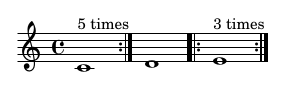
\includegraphics{../graphics/RepeatFollowedByANoteAndARepeat.png}

\caption{Three segments in a voice}
\label{Three segments in a voice}
\end{center}
\end{figure}


% -------------------------------------------------------------------------
\section{Notes and rests}\label{Notes and rests}
% -------------------------------------------------------------------------

\Class{msrNote} is complex class: it handles many variants, but using classes to represent the variants would be too cumbersone. As shown at \figureRef{The MSR classes hierarchy}:
\begin{itemize}
\item a note can be a standalone (regular) note or rest;
\item it can belong to a grace notes group;
\item it can belong to chord, which can itself belong to a grace notes group or a tuplet;
\item it can belong to a tuplet;
\item it can belong to double tremolo;
\item and finally, a rest can be unpiched.
\end{itemize}

\class{msrNote} thus uses enumeration type \enumType{msrNoteKind}, defined in \msr{msrBasicTypes.h}, to distinguish them:
\begin{lstlisting}[language=CPlusPlus]
enum class msrNoteKind {
  kNote_UNKNOWN_,

  // in measures
  kNoteRegularInMeasure,
  kNoteRestInMeasure,
  kNoteSkipInMeasure, // an invisible rest
  kNoteUnpitchedInMeasure,

  // in chords
  kNoteRegularInChord,

  // in tuplets
  kNoteRegularInTuplet,
  kNoteRestInTuplet,
  kNoteUnpitchedInTuplet,

  // in grace notes groups
  kNoteRegularInGraceNotesGroup,
  kNoteSkipInGraceNotesGroup, // used to circumvent LilyPond issue #34

  // in chords in grace notes groups
  kNoteInChordInGraceNotesGroup,

  // in tuplets in grace notes groups
  kNoteInTupletInGraceNotesGroup,

  // in double-tremolos
  kNoteInDoubleTremolo
};
\end{lstlisting}


%% -------------------------------------------------------------------------
%\section{Articulations}\label{Articulations}
%% -------------------------------------------------------------------------
%
%
%% -------------------------------------------------------------------------
%\section{Ornaments}\label{Ornaments}
%% -------------------------------------------------------------------------
%
%
%% -------------------------------------------------------------------------
%\section{Ties}\label{Ties}
%% -------------------------------------------------------------------------
%
%
%% -------------------------------------------------------------------------
%\section{Dynamics}\label{Dynamics}
%% -------------------------------------------------------------------------
%
%
%% -------------------------------------------------------------------------
%\section{Beams}\label{Beams}
%% -------------------------------------------------------------------------
%
%
%% -------------------------------------------------------------------------
%\section{Slurs}\label{Slurs}
%% -------------------------------------------------------------------------


% -------------------------------------------------------------------------
\section{Grace notes groups}\label{Grace notes groups}
% -------------------------------------------------------------------------

Grace notes groups handling is presented at \sectionRef{Grace notes groups handling}.


% -------------------------------------------------------------------------
\section{Chords}\label{Chords}
% -------------------------------------------------------------------------

A chord contains notes only, and can occur in measures, tuplets and grace notes groups, hence:
\begin{lstlisting}[language=CPlusPlus]
// chords
//______________________________________________________________________________

enum class msrChordInKind {
  kChordIn_UNKNOWN_,

  kChordInMeasure,
  kChordInTuplet,
  kChordInGraceNotesGroup
};
\end{lstlisting}


% -------------------------------------------------------------------------
\section{Tuplets}\label{Tuplets}
% -------------------------------------------------------------------------

Tuplets handling is presented at \sectionRef{Tuplets handling}.

A tuplet can contain:
\begin{itemize}
\item notes and rests;
\item chords;
\item other tuplets.
\end{itemize}

Tuplets can occur in measures and other tuplets, hence \enumType{msrTupletInKind}:
\begin{lstlisting}[language=CPlusPlus]
enum class msrTupletInKind {
  kTupletIn_UNKNOWN_,

  kTupletInMeasure,
  kTupletInTuplet
};
\end{lstlisting}

Tuplets factors are represented by \class{msrTupletFactor}, defined in\\
\msrBoth{msrBasicTypes}.
\begin{lstlisting}[language=CPlusPlus]
class EXP msrTupletFactor
{
	// ... ... ...

  public:

    // public services
    // ------------------------------------------------------

    Bool                  isEqualToOne () const
                              {
                                return
                                  fTupletActualNotes == fTupletNormalNotes;
                              }

    mfRational              asRational () const
                            {
                              return
                                mfRational (
                                  fTupletActualNotes,
                                  fTupletNormalNotes);
                            }

	// ... ... ...

  private:

    // private fields
    // ------------------------------------------------------

    int                   fTupletActualNotes;
    int                   fTupletNormalNotes;
};
\end{lstlisting}


% -------------------------------------------------------------------------
\section{Harmonies and figured bass similarities}\label{Harmonies and figured bass similarities}
% -------------------------------------------------------------------------

Harmonies and figured bass handling is presented at \sectionRef{Harmonies handling} and \sectionRef{Figured bass elements handling}, respectively.

In \mxml, harmonies and figured bass occur at the measure level:
\begin{lstlisting}[language=MusicXML]
      <harmony print-frame="no">
        <root>
          <root-step>C</root-step>
          </root>
        <kind text="m">minor</kind>
        </harmony>
      <note default-x="75.17" default-y="-35.00">
        <pitch>
          <step>F</step>
          <octave>4</octave>
          </pitch>
        <duration>2</duration>
        <voice>1</voice>
        <type>quarter</type>
        <stem>up</stem>
        </note>
\end{lstlisting}

\begin{lstlisting}[language=MusicXML]
      <harmony>
        <root>
          <root-step>F</root-step>
          <root-alter>1</root-alter>
        </root>
        <kind>major</kind>
        <inversion>2</inversion>
      </harmony>
      <note>
        <pitch>
          <step>C</step>
          <octave>4</octave>
        </pitch>
        <duration>4</duration>
        <type>whole</type>
      </note>
\end{lstlisting}

In MSR, the instances of \class{msrHarmony} and \class{msrFiguredBass} are present twice:
\begin{itemize}
\item each \class{msrNote} instance contains the harmonies and figured bass attached to it:
\begin{lstlisting}[language=CPlusPlus]
class EXP msrNote : public msrTupletElement
{
	// ... ... ...

  private:

    // private fields
    // ------------------------------------------------------

    // harmonies
    // ------------------------------------------------------

    std::list<S_msrHarmony>
                          fNoteHarmoniesList;

    // figured bass
    // ------------------------------------------------------

    std::list<S_msrFiguredBass>
                          fNoteFiguredBassesList;

	// ... ... ...
};
\end{lstlisting}

\item each \class{msrPart} instance contains a harmonies staff and voice, as well as a figured bass staff and voice:
\begin{lstlisting}[language=CPlusPlus]
class EXP msrPart : public msrPartGroupElement
{
	// ... ... ...

  private:

    // private fields
    // ------------------------------------------------------
   // harmonies

    S_msrStaff            fPartHarmoniesStaff;
    S_msrVoice            fPartHarmoniesVoice;

    // figured bass

    S_msrStaff            fPartFiguredBassStaff;
    S_msrVoice            fPartFiguredBassVoice;

	// ... ... ...
};
\end{lstlisting}
\end{itemize}

The way harmonies and figured bass elements are represented in \mf\ is presented in the next two sections.


% -------------------------------------------------------------------------
\section{Harmonies}\label{Harmonies}
% -------------------------------------------------------------------------

Harmonies handling is presented at \sectionRef{Harmonies handling}.


% -------------------------------------------------------------------------
\section{Figured bass}\label{Figured bass}
% -------------------------------------------------------------------------

Figured bass elements handling is presented at \sectionRef{Figured bass elements handling}.


% -------------------------------------------------------------------------
\section{Lyrics}\label{Lyrics}
% -------------------------------------------------------------------------

Lyrics handling is presented at \sectionRef{Lyrics handling}.

Lyrics are handled in rather a special way in music scores:
\begin{itemize}
\item they have a linear structure, independent of the repeats structure of the staff they belong too;
\item the can be several lyrics stanzas associated to a given staff;
\item the syllables in lyrics can apply to more that one note, and the subdivisions of words have to be handled.
\end{itemize}

The basic building block for lyrics in MSR is \class{msrSyllable}, whose variants are distinguished by enumeration type \enumType{msrSyllableKind}:
\begin{lstlisting}[language=CPlusPlus]
    enum class msrSyllableKind {
      kSyllableNone,
      kSyllableSingle,
      kSyllableBegin, kSyllableMiddle, kSyllableEnd,

      kSyllableOnRestNote,
      kSyllableSkipRestNote,
      kSyllableSkipNonRestNote,

      kSyllableMeasureEnd,
      kSyllableLineBreak, kSyllablePageBreak
    };
\end{lstlisting}

Extensions are described by enumeration type {\tt }:
\begin{lstlisting}[language=CPlusPlus]
    enum class msrSyllableExtendKind {
      kSyllableExtendNone,
      kSyllableExtendEmpty,
      kSyllableExtendSingle,
      kSyllableExtendStart, kSyllableExtendContinue, kSyllableExtendStop
    };
\end{lstlisting}

\Class{msrSyllable} contains:
\begin{lstlisting}[language=CPlusPlus]
    // syllable kind
    msrSyllableKind       fSyllableKind;

    // texts list
    std::list<std::string>
                          fSyllableTextsList;

    // extend kind
    msrSyllableExtendKind fSyllableExtendKind;

    // stanza number, may contain non-digits
    std::string           fSyllableStanzaNumber;

    // syllable whole notes
    mfRational              fSyllableWholeNotes;

    // syllable tuplet factor
    msrTupletFactor       fSyllableTupletFactor;
\end{lstlisting}

Syllables are one case where the data in MSR is denormalized: a given \class{msrSyllable} instance belongs both to an \class{msrNote} instance and to a lyrics instance of \class{msrVoice}.

At the higher level, syllables are organized as instances of \class{msrStanza}, which contains:
\begin{lstlisting}[language=CPlusPlus]
    // contents
    std::vector<S_msrSyllable> fSyllables;

    Bool                  fStanzaTextPresent;
\end{lstlisting}


% -------------------------------------------------------------------------
\section{MIDI}\label{MIDI}
% -------------------------------------------------------------------------

MIDI handling is presented at \sectionRef{MIDI handling}.
